% Metódy inžinierskej práce

\documentclass[10pt,twoside,slovak,a4paper]{article}

\usepackage[slovak]{babel}
%\usepackage[T1]{fontenc}
\usepackage[IL2]{fontenc} % lepšia sadzba písmena Ľ než v T1
\usepackage[utf8]{inputenc}
\usepackage{graphicx}
\usepackage{url} % príkaz \url na formátovanie URL
\usepackage{hyperref} % odkazy v texte budú aktívne (pri niektorých triedach dokumentov spôsobuje posun textu)

\usepackage{cite}
%\usepackage{times}

\pagestyle{headings}

\title{Využitie gamifikácie vo výučbe cudzích jazykov \thanks{Semestrálny projekt v predmete Metódy inžinierskej práce, ak. rok 2020/21, vedenie: Jozef Sitarčík}} % meno a priezvisko vyučujúceho na cvičeniach

\author{Peter Janoš\\[2pt]
	{\small Slovenská technická univerzita v Bratislave}\\
	{\small Fakulta informatiky a informačných technológií}\\
	{\small \texttt{xjanosp@stuba.sk}}
	}

\date{\small 20.8.2020} % upravte


\begin{document}

\maketitle

\begin{abstract}
Ovládanie cudzieho jazyka sa v dnešnej dobe považuje za nevyhnutné. Mnoho ľudí sa s cudzím jazykom, ako napríklad angličtina, stretáva už v ranom veku v školách a potom s ňou prichádzajú do kontaktu takmer každý deň na internete, v hudbe, vo filmoch alebo v článkoch, čo im pomáha sa ďalej rozvíjať. Existuje ale aj skupina ľudí, ktorí takéto možnosti nemali a chcú sa cudzí jazyk naučiť sami. No učenie sa cudzieho jazyka je zložitý proces a preto vznikli nové spôsoby vzdelávania, ktoré ho má zjednodušiť. Jeden z týchto nových spôsobov je takzvaná gamifikácia. Gamifikácia je relatívne nový koncept, ktorý spája zábavu s učením. Využíva herné elementy a dizajn, čo v teórii spríjemňuje atmosféru pri učení a taktiež odmieňa učiaceho sa za jeho pokroky, čo ho motivuje sa naďalej zlepšovať. Výsledky štúdií, ktoré sa venovali efektivite tejto stratégie ale preukázali zmiešané výsledky. V tomto článku sa budeme bližšie venovať gamifikácií ako takej, učeniu sa cudzieho jazyka a aj tomu ako môže táto stratégia pomáhať motivovať účastníka zapájať sa do tohto vzdelávacieho procesu.
\end{abstract}



\section{Úvod}

Hry sú súčasťou života mnohých ľudí. Aj preto môžeme čoraz častejšie vidieť, že sa nejakú formu hry snažia učitelia implementovať aj do vzdelávania. Takýmto spôsobom učenia sa je aj stále viac a viac populárnejšia gamifikácia, ktorej sa budeme venovať v tomto článku. Gamifikácia, by mohla byť novou metódou, ktorá by umožňovala učiteľom viac motivovať svojich študentov, aby sa efektívnejšie a rýchlejšie naučili druhý jazyk. 

Keďže je gamifikácia stále relatívne novým konceptom, nebolo na ňu vykonaných veľa štúdií, ktoré by potvrdzovali alebo vyvrátili jej efektívnosť.

\section{Nejaká časť} \label{nejaka}

Z obr.~\ref{f:rozhod} je všetko jasné. 

\begin{figure*}[tbh]
\centering
%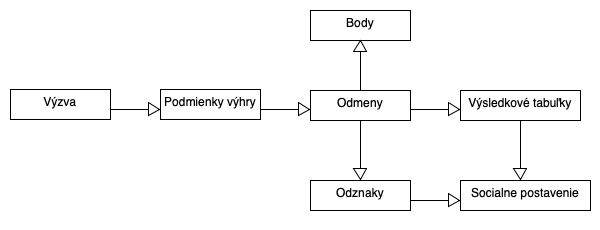
\includegraphics[scale=1.0]{diagram.pdf}
Aj text môže byť prezentovaný ako obrázok. Stane sa z neho označný plávajúci objekt. Po vytvorení diagramu zrušte znak \texttt{\%} pred príkazom \verb|\includegraphics| označte tento riadok ako komentár (tiež pomocou znaku \texttt{\%}).
\caption{Rozhodujúci argument.}
\label{f:rozhod}
\end{figure*}



\section{Iná časť} \label{ina}

Základným problémom je teda\ldots{} Najprv sa pozrieme na nejaké vysvetlenie (časť~\ref{ina:nejake}), a potom na ešte nejaké (časť~\ref{ina:nejake}).\footnote{Niekedy môžete potrebovať aj poznámku pod čiarou.}

Môže sa zdať, že problém vlastne nejestvuje\cite{Coplien:MPD}, ale bolo dokázané, že to tak nie je~\cite{Czarnecki:Staged, Czarnecki:Progress}. Napriek tomu, aj dnes na webe narazíme na všelijaké pochybné názory\cite{PLP-Framework}. Dôležité veci možno \emph{zdôrazniť kurzívou}.


\subsection{Nejaké vysvetlenie} \label{ina:nejake}

Niekedy treba uviesť zoznam:

\begin{itemize}
\item jedna vec
\item druhá vec
	\begin{itemize}
	\item x
	\item y
	\end{itemize}
\end{itemize}

Ten istý zoznam, len číslovaný:

\begin{enumerate}
\item jedna vec
\item druhá vec
	\begin{enumerate}
	\item x
	\item y
	\end{enumerate}
\end{enumerate}


\subsection{Ešte nejaké vysvetlenie} \label{ina:este}

\paragraph{Veľmi dôležitá poznámka.}
Niekedy je potrebné nadpisom označiť odsek. Text pokračuje hneď za nadpisom.



\section{Dôležitá časť} \label{dolezita}




\section{Ešte dôležitejšia časť} \label{dolezitejsia}




\section{Záver} \label{zaver} % prípadne iný variant názvu



%\acknowledgement{Ak niekomu chcete poďakovať\ldots}


% týmto sa generuje zoznam literatúry z obsahu súboru literatura.bib podľa toho, na čo sa v článku odkazujete
\bibliography{literatura}
\bibliographystyle{plain} % prípadne alpha, abbrv alebo hociktorý iný
\end{document}
